\chapter{Background}
\label{chapter:chapter02}

\section{Optimality}

There are two different interpretations of optimality one refers to Single-Objective Optimisation and the other to Multi-Objective Optimisation\\

\subsection{Single-Objective Optimisation}

A general Single-Objective Optimisation problem is defined as \textit{minimising or maximising a function $f(x)$ subject to $g_i(x) \essoreq 0$ and $h_j(x) = 0$ of some universe $\Omega$. A solution minimises or maximises the scalar f(x) where $x$ is a n-dimensional decision variable vector $x = (x_1,...,x_n)$.}\\
 
Here $g_i(x)$ and $h_j(x)$ refers to the constraints that must be fulfilled while optimising $f(x)$. $\Omega$ is the Universe representing all the acceptable solutions possible that can be used to satisfy $f(x)$ and its constraints. The $x$ decision vector can be whether continuous or discrete variables and its evaluation $f$ can also be continuous or discrete as well.\\

Single Objective Global Minimum Optimisation is defined as \textit{Given a function $f: \omega \subseteq \mathbb{R}^n \rightarrow \mathbb{R}, \Omega \neq 0$ for $x \in \Omega$ the value $f* \triangleq f(x^*) > -\infty$ is called a \textbf{global minimum} if and only if}\\

\begin{equation}
    \forall x \in \Omega: f(x^*) \leq f(x).
\end{equation}

\textit{$x^*$ is by definition the global minimum solution, $f$ is the objective function, and $\Omega$ represents all the possible values of $x$. The goal of determining the global minimum solution is called the \textbf{global optimisation problem} for a single-objective problem.}\\

\subsection{Multi-Objective Optimisation}

For multi-objective optimisation, is not possible to compare two solutions $x$ and $y$ directly, the quality of the solutions is therefore compared by their dominance.\\

\subsubsection{Dominance}

A solution $a_i$ of a set $A = (a_1,...,a_n)$ is said to \textit{dominate} a solution $b_i$ of another set $B = (b_1,...,b_n)$, denoted by $a_i \pred b_i$ or $f(x) \pred f(y)$ with, if and only if $a_i$ is at least as optimal as $b_i$ in all objectives of $b_i$ and with at least one of its objectives better than $b_i$.\\

In multi-objective optimisation, the goal is to find the set of optimal solutions, known as the Pareto optimal set. Pareto optimality is defined concerning the concept of non-domination between the points of the objective space $\Omega$ if and only if there is no vector in the set $A$ that results better in set $B$. This is known as the \textbf{Pareto optimal Set}, formally speaking, for a given MOP, the \textbf{Pareto Optimal set} is represented as:

\begin{equation}
    P* := \{x \in \Omega | ¬\exists x' \in \Omega f(x') \predeq f(x) \}
\end{equation}

A Pareto optimal set is composed of optimal solutions, which its internal objectives cannot be improved simultaneously. Their corresponding vectors are termed as \textit{non-dominated}, the collection of Pareto optimal solutions being the result of the same MOP receive the name of \textbf{Pareto Front} where:
\begin{equation}
    PF* := \{u= F(x) | x \in P*\}
\end{equation}


\section{Evolutive Algorithms}

Los algoritmos evolutivos forman parte de la computación evolutiva, son algoritmos basados en una población meta-heurísticos para resolver problemas de optimización. Un algoritmo evolutivo usa mecanismos inspirados en la evolución biológica como pueden ser la reproducción, mutación, recombinación y selección, las soluciones candidatas a la optimización forman parte de una población y una función de ajuste determina la calidad de cada una de estas soluciones. Este ajuste toma parte después de distintas iteraciones o generaciones en las que se busca acercarse lo más posible a la función objetivo.[10] \\

Usualmente este tipo de algoritmos tiene un buen desempeño, ya que no se encuentran influenciados directamente por una función de ajuste, la única que interacción que tienen con ésta resulta ser la de un filtro para definir las poblaciones subsecuentes. El uso de estos algoritmos para el modelado de la evolución biológica se limita únicamente a la exploración de micro-evolución o la determinación de sistemas de procesos celulares, por lo que suelen ser más comúnmente usados en problemas donde la complejidad computacional resulta un factor prohibitivo. De hecho la complejidad computacional se deriva directamente de la función de ajuste. La aproximación a esta función es una de las soluciones que supera esta dificultad. [11] \\

En este proceso hay dos fuerzas fundamentales que forman la base de los sistemas evolutivos: \\
\begin{itemize}
\item Los operadores de variación (que son de recombinación y mutación) crean la diversidad necesaria y por lo tanto facilitan la posibilidad de encontrar nuevas soluciones.
\item La selección actúa como una fuerza que empuja la calidad.
\end{itemize}

Los algoritmos evolutivos poseen un número de características que pueden ayudar a posicionarse dentro de las familias de métodos de generación y prueba:

\begin{itemize}
\item Son basados en poblaciones, esto significa que procesan una cantidad variable de soluciones candidatas de forma simultánea.
\item Usualmente usan una recombinación para mezclar la información de más candidatos en soluciones nuevas.
\item Estos algoritmos son estocásticos.
\end{itemize}


Un algoritmo evolutivo generalmente cuenta con los siguientes componentes:

\begin{itemize}
\item Representación (definición de las soluciones)
\item Función de evaluación (o función de ajuste)
\item Población
\item Selección de padres
\item Operaciones de variación, recombinación y mutación
\item Mecanismo de selección de sobrevivientes 
\end{itemize}


Cada uno de estos componente se deben de ser especificados para definir un algoritmo en particular, por lo tanto la inicialización del algoritmo tanto como la condición de terminación deben de ser definidas también.[11]

A continuación se describen los pasos que lleva a cabo un algoritmo evolutivo comúnmente:

\begin{itemize}
\item \textbf{Inicialización}: Se generan distintas soluciones de forma aleatoria
\item \textbf{Evaluación}: Cada una de las soluciones pasa a ser evaluada por la función de ajuste y se determina que tanto se acerca a su valor óptimo
\item \textbf{Terminación}: Se determina si se alcanzó el objetivo con alguno de los candidatos o si se sobrepasó el número de generaciones límite que se estableció previamente.
\item \textbf{Selección}: Se selecciona las soluciones que "sobreviven" y pasan a la siguiente generación
\item \textbf{Variación}: este paso puede darse por medio de del paso de "cromosomas" o características de las soluciones que sobrevivieron en el paso anterior para combinarse entre sí y dar nuevas soluciones "hijas", el otro método es la mutación, donde una o varias de las características se modifica de manera aleatoria para introducir un nuevo valor a la población
\end{itemize}

Este ciclo se repite dando paso cada vez a nuevas generaciones que cada vez se ajustan más a la función de evaluación hasta que se alcance el resultado deseado determinado por el paso de Terminación.[10] \\

\section{Single-Objective Algorithms}
% INSERT: Brief introduction to the algorithms used, explaining that at the beginning a lot more were considered but were discarded since the problem is discrete (there can only be the students that are present in the dataset, there aren't new students created on the fly)

% REMINDER: Here are only the definitions of each of the algorithms the specific implementation will be defined in the experimentation phase.

% Most of the definitions are taken from doi.org/10.1016/j.ins.2013.02.041 but further descriptions are taken from this article sources.

La optimización mono-objetivo o optimización global es un tipo de problemas que consiste en encontrar el mínimo o el máximo global de una función, ya que en una función no lineal pueden haber mínimos locales, pero un mínimo global es más difícil de encontrar, también es importante tomar en cuenta que se considera un dominio de soluciones y otras limitantes, por lo que en general la solución más obvia suele ser realizar una búsqueda exhaustiva probando cada uno de los valores del dominio, sin embargo esta estrategia puede llegar a ser bastante ineficiente. En los problemas no lineales una función puede contener un número muy largo de máximos y mínimos, a estos se les denominan mínimos o máximos locales, y para encontrarlos basta con usar un método local de optimización clásico.[1], [7], [8] \\

Los algoritmos para encontrar un mínimo global comprenden métodos exactos y heurísticos. Dentro de los algoritmos exactos existen La búsqueda exhaustiva, búsquedas bayesianas, aproximaciones sucesivas y algunos algoritmos estocásticos como el muestreo de Monte-Carlo en el cual una simulación aleatoria es usada para encontrar una solución aproximada, Tuneleo estocástico, etc.[7] \\

\subsection{Local Search}
 
Also referred as Hill Climbing in maximisation problems and Steepest Descent in minimization problems, the definition of this algorithm is taken from [doi.org/10.1016/j.ins.2013.02.041] here it is accredited to Stutzle in his PhD dissertation who actually does not take credit for this approach and instead mentions specific instances of the algorithm included in the literature.\\

Local Search is a single objective optimisation meta-heuristic based on the idea of generating random starting solutions, then in each generation, LS generates the starting solution for the next iteration by perturbing the local optimum found in the current iteration. \\

It is important to mention that the perturbing mechanism is an important feature of LS, since a weak perturbation may not be enough to escape the local optimum, and on the other hand a too strong perturbation may make the algorithm too similar to a multi-start local search with randomly generated starting solutions. \\

A pseudo-code for this algorithm can be seen in the algorithm. \ref{local_search_alg}

\begin{algorithm}[H]
\label{local_search_alg}
\caption{Local Search Algorithm}
\SetAlgoLined 
 Choose, at random, an initial solution $s$ in the search space\;\\
 Apply a local search starting from $s$ to get a solution $s*^$\;\\
 \Repeat{the stopping criterion is satisfied}{
  Perturb $s^*$ to get a solution $p$\;\\
  Apply a local search starting from $p$ to get a solution $p*$\;\\
  \eIf{the acceptance criterion is satisfied}{
   $s^*$ \gets $p^*$\;
  }
 }
 \textbf{return} the best solution met\;
\end{algorithm}


\subsection{Genetic Algorithms}

This is probably the most known kind of metaheuristic for optimization, it was developed in the early '70s in Michigan with John Hoolland and some of his students who were researching adaptive systems at the time. [https://doi.org/10.1016/j.ins.2013.02.041].\\

The definition can be very generic an most of its parts are usually implemented differently according to each problem. Its essential parts include a representation of the solution known as Chromosome, a selection strategy a type of cross-over and a mutation operator.\\

The Chromosome is a representation of the solution and usually includes inside of it a string of genes, most commonly represented as a fixed binary string, although it can also be represented by any kind of value for combinatorial problems. A mutation is therefore done by changing a single gene to a different value, performing a bit-flip in the case of the binary representation, for example.\\

Crossover is a recombination of the genes, usually done with 2 individuals, which exchange their parts to create a new individual, this follows different strategies such as the n-point crossover in which a point will determine which parts will be inherited from one of its parents and which from the other. An external parameter known as $pc$ (crossover rate) indicates the probability of each individual to undergo crossover, this value ranges from 0.6 to 1.0 according to []\\
% [13 in https://doi.org/10.1016/j.ins.2013.02.041]. 

Individuals that can produce offspring are then chosen using a selection strategy after the fitness of each individual has been evaluated. The most common selection scheme is the roulette-wheel selection, but other types of selections such as tournament selection and ranking selection are also common.\\

After the crossover, the individuals are subjected to mutation. This mutation procedure introduces some kind of randomness which in essence introduces new genes in the solution, this is to prevent being trapped into the local optima. This operator is usually used with a small probability, as low as $1\%$, according to [Article], but the appropriate mutation rate is still an open issue.\\

Finally, the replacement or survivor selection uses the fitness value to identify the individuals which will serve as the parents for the next generations and is responsible to assure the survival of the fittest individuals.\\

An example of an implementation of a $GA$ can be seen in algorithm\ref{genetic_alg}.

\begin{algorithm}[H]
\label{genetic_alg}
\caption{Genetic Algorithm}
\SetAlgoLined 
Generate Initial population $p$\;\\
Compute fitness of each individual\;\

\Repeat{stopping condition has been met}{
    \textit{Produce a new generation}\;\\
    \For{size of $p$ / 2}{
        Select two individuals from the previous generation for matching\;\\
        Recombine the two individuals to give two new off springs\;\\
        Insert the offspring in the new generation\;\\
    }
}
 \textbf{return} the best solution met\;
\end{algorithm}

\subsection{Evolution Strategy}

Similar to the Genetic Algorithms, described in the last section, these algorithms try to follow the principles of natural evolution as their method to solve optimization problems. They were introduced during the 0's by Rechenberg [216, 217] and further developed by Schwefel later. The first algorithm used in experimentation was Two membered ES and had a simple mutation-selection scheme.

The basic structure consists of a single parent which produces an offspring following a normally distributed mutation resulting in a $\lambda$ number of individuals. Next, a selection operator determines the fittest individual which then becomes the parent of the next generation.

The selection process resembles an "extinction of the worst", which means the less fitted individuals are replaced, which sometimes may include the parents, the population is kept with the size $\lambda$ constantly in each of the generations.\\

At the time of its conception, the idea of a population wasn't widely used so far, which is why Rechenberg proposed a multi-member ES in [(probably 216 or 217)] where more than one parent can participate in the generation of one offspring individual. This is denoted as $(\mu + 1) - ES$ where $\mu$ represents the number of parents.\\ 

Two other definitions were then introduced by Schwefel in [237 from the article], which were $(\mu + \lambda) - ES$ and $(\mu, \lambda) - ES$.\\

\begin{itemize}
    \item $(\mu + \lambda) - ES$, known as Elitist Evolution Strategy, indicates that $\mu$ parents will create $\mu \geq 1$ descendants by recombination and mutation, keeping the best-fitted individual of the previous generation and discarding the rest
    \item $(\mu, \lambda) - ES$, known as Non-Elitist Evolution Strategy, is similar with the difference that none of the parents is kept in any of the subsequent generations, disregarding how good or bad was its fitness compared to the generation they belong.
\end{itemize}\\

Two other well-known ES is $(\mu/\rho + \lambda) - ES$ and ($\mu/\rho, \lambda) - ES$, where the $\rho$ refers to the number of parents involved in the procreation the offspring. Mutation in ES can be realised through normally distributed numbers with a mean of $0$ and $a$ standard deviation of $\sigma$, which represents the size in the mutation step when the problem has a continuous solution.

A basic version of the Evolution Strategy can be seen in \ref{evolution_alg}

\begin{algorithm}[H]
\label{evolution_alg}
\caption{Evolution Strategy Algorithm}
\SetAlgoLined
    \textit{Initialize} the population with random individuals\;\\
    \textit{Evaluate} each individual
    \Repeat{the termination condition is satisfied}{
        \textit{Select} parents\;\\
        \textit{Recombine} pairs of parents\;\\
        \textit{Mutate} the resulting offspring\;\\
        \textit{Evaluate} new individuales\;\\
        \textit{Select} individuals for the next generation\;\\
    }
\end{algorithm}

\subsection{Random search} 

Also known as Pure Random Search was first defined by Brooks in ... 
% [https://www.jstor.org/stable/167616?seq=1#page_scan_tab_contents]
and later named in the classic volumes by Dixon and Szego [44, 45 (from  https://link.springer.com/book/10.1007/978-1-4419-9182-9)].

It is considered as one of the most basic search strategies. It consists of the following: in each step, it creates a new random solution, and the best solution is updated if the new solution outperforms the fit value of the previous best solution.

While this algorithm sacrifices the guarantee of determining the optimal solution within the search space, it can be shown that a pure random search converges to the global optimum with a probability of 1.0 according to [https://link.springer.com/book/10.1007/978-1-4419-9182-9].

This is most commonly used in addition to other search algorithms compare its performance to random sampling according to [http://sci-hub.tw/https://doi.org/10.1002/spe.2459].

\subsection{Random Descent} 

Also known as Stochastic Hill Climbing. It is an algorithm similar to regular Hill Climbing, with the difference that it includes a neighbourhood which limits the search to only the solutions that are close to the current best solution in each step.

Perhaps the most popular implementation of it was done by Forrest and Mitchell naming it Random Mutation Hill Climbing (RMHC) algorithm (with communication from Richard Palmer) [M. Mitchell and J. H. Holland, "When Will a Genetic Algorithm Outperform Hill Climbing?", in Proceedings of the 5th International Conference on Genetic Algorithms, 1993.]

The local improvements are determined by a neighbourhood structure and a fitness function on the search space of the algorithm. This neighbourhood structure can be seen as an undirected graph G on vertex set S. The algorithm checks a member of its neighbourhood randomly and transitions to this solution when there is an improvement in the fitness function result or it is the same, the process is then repeated in each step.

It was designed with discrete domains in mind, since they have explicit neighbourhoods, such as with combinatorial optimization problems. However, even being a stochastic optimization process, it can still get stuck in a local optimum.

\begin{algorithm}[H]
\label{evolution_alg}
\caption{Pseudocode for stochastic hill climbing}
\SetAlgoLined
    Currrent solution $s$ from new population\;\\
    Evaluate the objective function $f(s)$\;\\
    $stop = \textit{FALSE}$\;\\
    $iter = 0$\;\\
    \While{$stop = \textit{FALSE}$}{
      Choose a random solution in the neighbourhood $s_n$\;\\
      \eIf{$f(s_n) > f(s)$}{
        replace $s$ by $s_n$\;
       }{
        $iter = iter + 1$\;
      }
      \eIf{$iter = iter_{max}$}{
        $stop = TRUE$\;
      }
     }
\end{algorithm}

\subsection{Parallel Tempering (Replica Exchange Monte Carlo)} 

It's an algorithm Also known as Replica Exchange Monte Carlo It is considered Similar to Simulated Annealing since it also uses the concept of temperatures, but it has the advantage that takes advantage by using a multi-core architecture. [http://www.jamesframework.org/docs/].

It was originally mentioned as a simulation technique known as replica exchange in a paper by Swendsen and Wang.1. In this paper, a method of replica Monte Carlo was introduced in which replicas of a system of interest were simulated at a series of different temperatures. Then these replicas undergo a partial exchange of configuration information. The more general form of parallel tempering with a complete exchange of configuration information was introduced in 1991 by Geyer according to [doi.org/10.1039/B509983H].

This algorithm runs several replicas of a particular system of interest, using different temperatures in each one of them. High temperature can generate large volumes of phase spaces, while low-temperature systems tend to have more precision in the sampling of the phase space and tend to be trapped in a local optimum.

This particular implementation of the algorithm uses Metropolis search as the system to replicate, which is an extension of Random Descent where Metropolis where a valid neighbour that is no improvement over the current solution may still be accepted as the new current solution, and the probability to accept an inferior neighbour is proportional to the difference in the evaluation of the current solution and the temperature of the search.

Using this algorithm requires a minimum and maximum temperature, with each replica of the system with an assigned temperature, after each step the replicas are ordered according to their temperature, and then swapped to push the better solutions to the lowest temperatures, so they can eventually converge while higher temperature replicas are constantly modified in a search for improvement. Each of the replicas applies repeatedly a series of moves to a private solution, and then the global solution is tracked in the main search.
\begin{algorithm}[H]
\label{parallel_temp_alg}
\caption{Parallel Tempering}
\SetAlgoLined
\For{$i \gets 0$ \textbf{to} $M - 1$}{
    $T_i \gets$ calculate temperature $i$\;\\
    $replica_i \gets$ new instance of Metropolis search with temperature $T_i$
}
\Repeat{The stop criterion has been met}{
    \For{$i \gets 0$ \textbf{to} $M - 1$}{
        Run $replica_i$ for $N_{swap}$ iterations
    }
    $G \gets min(Cost({global_best}_{replica(0)},...,Cost({global_best}_{replica(M - 1)})))$\;\\
    $j \gets U\{0,M-1\} \Comment{Randomly select adjacent temp. levels}$\;\\
    $\Delta E \gets (Cost({active\_solution}_{replica(j)}) - Cost({active\_solution}_{replica(j + 1)}))/G$\;\\
    $\Delta \beta \gets 1/{T_j} - 1/{T_{j+1}}$\;\\
    \eIf{$U(0,1) < min(1,exp(\Delta E\Delta \beta))$}{
        Set the temp. of $replica_j$ and $replica_{j+1}$ to $T_{j+1}$ and $T_j$, respectively\;\\
        $swap($replica_j$,$replica_{j+1}$)$ \Comment{Keeps replicas ordered by temp.}
    } 
}
\end{algorithm}

\section{Multi-Objective Algorithms}

La optimización multiobjetivo es un área del análisis de decisión de múltiples criterios que se encuentra directamente relacionada con los problemas de optimización matemática, que involucra más de una función objetivo para que sea optimizada simultáneamente. [4] \\

Estas soluciones pueden tener distintos criterios o características para ser consideradas opciones óptimas, por lo que se les denominan soluciones de pareto. Una solución Óptima de Pareto se define como una solución cuyas funciones objetivo pueden ser mejoradas sin degradar el resto de las funciones. Se refiere a una solución no dominada en el espacio de criterio del problema. \\

Para los problemas de optimización multiobjetivo no triviales no existe una solución ideal óptima, sino que existen distintas soluciones que optimizan simultáneamente cada objetivo, en cuyo caso se dice que las funciones son contradictorias y existe un número de soluciones óptimas de Pareto. Todas las soluciones que son óptimas por Pareto se dice que son igualmente buenas para los objetivos que se hayan determinado.[4], [5] \\

Usualmente la idea de resolver un problema multiobjetivo es entendido como ayudar a un tomador de decisiones a considerar múltiples objetivos simultáneamente y encontrar una solución óptima de pareto que a su discreción sea más adecuada. Por lo que el método para encontrar la solución requiere de un involucramiento del tomador de decisiones y es influenciado fuertemente por sus preferencias. Usualmente en este tipo de problemas solo se toma en cuenta un sólo tomador de decisiones pero también existe la posibilidad de múltiples tomadores de decisiones. [9]

Stands for Electrostatic Potential Energy Evolutionary Algorithm and its and its a very recent algorithm that generates several Pareto front approximations, focusing only on the solutions that appear interesting to the decision-maker. Proposed in []
% https://sci-hub.se/https://dl.acm.org/citation.cfm?id=2754674
by [Authors]. It was proposed because it was noticed that many of the algorithms found in the literature make use of popular crowding distance metrics that don't necessarily converge into optimality according to [13 from https://sci-hub.se/https://dl.acm.org/citation.cfm?id=2754674]. It also has been shown in [28 from https://sci-hub.se/https://dl.acm.org/] that an optimal distribution depends on the chosen reference point, but these methods are not adequate for constrained problems or discontinuous Pareto fronts.\\

The algorithm attempts to design an electromagnetism inspired heuristic, each solution has an assigned charge based on how close it is to a randomly selected subset from an archive of non-dominates solution. Then the charges are translated to force vectors which move the solutions in the search space. The best solutions are stored in an archive that uses clustering and crowding distance to prune the solutions.\\

\begin{algorithm}[H]
\label{espea_alg}
\caption{ESPEA}
\SetAlgoLined
\Begin{
    Generate initial population $P$\;\\
    Copy all non-dominated solutions in $P$ to archive $A$\;\\
    \Repeat{stop criterion has met}{
        Generate a single new solution \textbf{$p$}\;\\
        Remove all solutions from $A$ dominated by $p$\;\\
        \eIf{$\textbf{p} \nsucc \textbf{a} \wedge \textbf{f(p)} \neq \textbf{f(a)} \forall \textbf{a} \in A$}{
            \eIf{$|A| < N$}{
                $A:= A \cup {p}$
            }{
                Calculate $e(a)$ for all $a \in \A$\;\\
                Calculate $e:= (e_{a^1}(p),...,e_{-a^N}(p))$\;\\
                $update(A,p,e)$
            }
        }
    }
}
\textbf{return $A$}
\end{algorithm}

% where e represents the energy

\subsection{MOMBI2}

MOMBI stands for Many Objective Metaheuristic Based on the $R2$ indicator introduced first in [https://sci-hub.se/10.1145/2739480.2754776] by Carlos A. Coello. It has an advantage over other many-objective optimization algorithms found in the literature since a lot of them such as NSGA-II relies on the Hypervolume indicator which can be become a costly function as the number of objectives grow, MOMBI2 uses the $R2$ indicator instead [8 from the article]. 

The $R2$ indicator is considered part of the $R$ indicator family first introduced by Hansen and Jaszkiewicz in 1998 [5 from http://www.cmapx.polytechnique.fr/~dimo.brockhoff/publicationListFiles/twb2013a.pdf]. All of them are based on a set of utility functions, in this case comparing 2 sets of points being a reference Pareto front and another front,  having several variants introduced at the time, with the variation being the way the utility functions are evaluated and combined:
\begin{itemize}
    \item $R1$, The ratio of the set is better than the other
    \item $R2$, The mean difference in utilities
    \item $R3$, The mean relative difference of in utilities
\end{itemize}

In particular, the $R2$ definition has been broadly used and is one of the most recommended performance indicators [8 from the article] along with Hypervolume and it is highly correlated to it [https://sci-hub.se/10.1145/2739480.2754776].

$R2$ is used because it induces the complete ranking in the set of all approximations. It is based on the assumption that it is allowed to add values of different utility functions in the set. Therefore it is also dependent on the scaling of its utility functions [https://sci-hub.se/10.1145/2739480.2754776].

The first version of MOMBI was introduced in [9 of https://sci-hub.se/10.1145/2739480.2754776] but it had the problem that it presented a loss of diversity in the solutions as the dimensions of the problem grew to address this problem the Chevishev function CHE set was changed to  the Achievement Scalarizing Function ASF which is similar to the former but introduces some normalisation.

The algorithm works as follows, each iteration new individuals are created from the parents selected randomly  here the looking for those individuals that minimised ASF

The maximum values of each objective function constitute a point $zmax$, it is ensured that there are not repeated individuals and the size of the population is at least the desired size, if these requirements are not satisfied, then the $zmax$ point is penalised by updating it with the worse values of the whole population.

In the following steps, the population is ranked and then reduced to the desired size.

\begin{algorithm}[H]
\label{mombi2_alg}
\caption{MOMBI2}
\SetAlgoLined
\textbf{Require:} MOP, stopping criterion,set of weight vectors $W$\;\\
\textbf{Ensure:} Pareto set approximation\;\\
Initialize population $P_i,i \gets 1$\;\\
Evauate population $P-i$\;\\
Calculate the $L_2-norm$ of objectives for $P_i$\;\\
Set $\vec z^{min} \gets \vec z^*$ and $\vec z^{max} \gets \vec z^{nad}$\;\\
\While{termination condition is not fulfilled}{
    Perform parent selection\;\\
    Generate offspring $P_i'$ using variation operators\;\\
    Evaluate population $P_i'$\;\\
    Calculate the $L_2-norm$ of objectives for $P_i'$\;\\
    Normalize objective functions for $P_i \cup P_i'$\;\\
    Execute $R2$ ranking algorithm $(P_i \cup P_i',W)$\;\\
    Reduce population $P_{i+1} \gets \{P_i \cup P_i'\}$\;\\
    Update reference points $(\vec z^{min},\vec z^{max},P_{i+1},m)$\;\\
    $i \gets i + 1$
}
\textbf{return} $P_i$
\end{algorithm}

% There are the algs for updating the reference points and the R2 rankings in https://sci-hub.se/10.1145/2739480.2754776, but I'm not sure if they should be included here.

\subsection{NSGAII}

NSGA-II

%Mostly taken from [https://www.iitk.ac.in/kangal/Deb_NSGA-II.pdf]
Is one of the most known Multi-Objective optimization methods, it was first proposed by Shinivas and Deb in 1994 for its first version, and then later in 2002 as NSGA-II following the work from Shinivas and other authors, this algorithm heavily relies on the concept of dominance introduced in section [ref]. Besides it also makes use of the Crowding Distance which is a certain preference for solutions that are less crowded in the solution space.

NSGAII was introduced as a response after the criticism of the first version NSGAII, which had the following problems, each one which has been addressed in this new version:

A high computational complexity of the non-dominated sorting, which had a complexity of $O(MN^3)$, where M is the number of objectives and N is the size of the population, this new version has instead a complexity of $O(M(2N)^2)$, the algorithm for this is shown in [fig]. Another problem was the lack of elitism, since [25], [18] have shown that elitism can speed up the performance of the GA significantly, the elitism as described in the next paragraph is now assured by keeping all the solutions from the previous generation when the ranking is done. Finally a need for specifying a sharing parameter, since traditional mechanisms use the concept of sharing to keep a wide variety of equivalent solutions.

This algorithm works as follows:

After an initial population is created, each individual is ranked and sorted according to their dominance, each solution then is assigned a fitness according to their non-domination level (1 is assigned to the best, then 2 and so on). This for minimisation problems. Then a binary tournament selection, crossover and mutation take place and an offspring population of size N is created, the process is then repeated joining the previous generation and their offspring as the same population, and it continues with the population always taking the parents of the previous generation, therefore Elitism is ensured. Is important to notice that in the following generations, the ranking will also consider the crowding distance for the ranking.

\begin{algorithm}[H]
\label{nsgaii_alg}
\caption{NSGAII}
\SetAlgoLined
Generate a random initial population $P_t$\\
$R_t \gets P_t \cup Q_t$ \Comment{combine parent and offspring population}\\
$F \gets fast-non-dominated-sort(R_t)$ \Comment{run the fast non dominates sort procedure and collect $F = (F_1,F_2,...)$ with the nondominated fronts of $R_t$}\\
$P_{t+1} = 0$ and $i = 1$\\
\Repeat{$|P_{t+1}| + |F_i| \leq N$ \Comment{until the parent population is filled}}{
    $crowding-distance-assigment(F_i)$ \Comment{calculate crowding-distance in $F_i$}\\
    $P_{t+1} = P_{t+1} \cups F_i$\\
    $i = i + 1$
}
$Sort(F_i, \prec_n)$\\
$P_{t+1} = P_{t+1} \cups F_i[1:(N-|P_{t+1}|)]$\\
$Q_{t+1} = make-new-pop(P_{t+1})$\\
$t = t+1$\\
\end{algorithm}


\subsection{RandomSearch}

Multi-Objective Random search is a probabilistic algorithm that, serves mostly as an algorithm to benchmark other optimization algorithms in the literature[https://sci-hub.se/10.1007/BFb0056872], just like its single objective counterpart, this produces a random set of solutions in each step. 

It considers the rate of crossover and mutation, but none is performed, so the number of evaluations will be the same as for the other EA's. The output of the algorithm is the Pareto-optimal set of all solutions generated.

\subsection{SPEA2}

SPEA \textbf{Strength Pareto Evolutionary Algorithm} first introduced by Zitzler and Thiele in 1999, was among the first techniques that were extensively compared to several existing evolution-based methods (Zitzler
and Thiele 1999; Zitzler, Deb, and Thiele 2000) according to [Coello's Book].

It makes use of an external non dominated set, for each individual in this set a strength value is computed, this consist of the raw fitness value assigned from the objective functions and a density estimation similar to the ranking value of MOGA[504 from Coello's book]. The algorithm applies the respective selection, crossover and mutation operators to fill an archive of individuals, then applies this fitness function and the non-dominated individuals from both the original population and the archive are copied into a new population. If the number of non-dominated individuals is greater than the population size, a truncation operator based on the distance to the k-nearest neighbour is used. Hence the individuals having the minimum distance to every other are discarded. Pareto dominance is used to ensure that the solutions are properly distributed along the Pareto front.

SPEAII introduced in [https://www.research-collection.ethz.ch/bitstream/handle/20.500.11850/145755/eth-24689-01.pdf] is different from its predecessor SPEA, has 3 main differences, it incorporates a fine-grained fitness assignment strategy that considers the number of individuals for each individual that dominates each one of them and the number of individuals that are dominated by each one of them too. It also uses a nearest neighbour density estimation strategy that makes the search more efficient. And it has an enhanced archive truncation strategy that guarantees the preservation of boundary solutions.

\textbf{Considering the fitness assignment}, the individuals that are dominated by the same archive members have identical fitness values. Which means that in case that the archive has only one individual all population members will have an independent rank value, therefore lowering the selection pressure and making SPEA behave like a random search algorithm.

\textbf{For the density estimation}, If many individuals are indifferent to the current generation, which means there is no domination between them, there is little to no information that can be obtained from them, which happens rather frequently, density information is used to guide the search more effectively. Clustering makes use of this information but only regarding the archive and not the population.

\textbf{Archive Truncation} considers that, while in SPEA the clustering technique was able to reduce the non-dominated set without destroying its features, it could lose outer solutions, however, these solutions must be kept in the archive to keep the spread of non-dominated solutions.

The algorithms work as follows:

First, all non dominated members are copied to the archive, if there is any dominated individual or a duplicate (with the same objective function evaluation), then they are removed from it during the update operation. If the size of the updated archive exceeds the predefined limit, further members are removed by a clustering technique which preserves the features of the non-dominated front. 

Then the fitness values are assigned to the archive and the population members. 
\begin{itemize}
    \item Each individual $i$ is assigned a strength value $S(i) \in [0, 1)$, which  at the same time considers the fitness function $F(i)$. $S(i)$ is the number of population members $j$ that are dominated or equal to i, divided by the population plus one.
    \item The fitness $F(j)$ of an individual $j$ in the population is calculated by summing the values of $S(i)$ of the rest of the archive members that dominate or are equal to $j$ plus one.
\end{itemize}

Then for the mating selection, individuals are selected by binary tournaments. This assumes a minimisation, each member of the archive has a higher chance of being selected than the rest of the population. Finally, after crossover and mutation operators are applied, the population is replaced by the resulting offspring population.

\begin{algorithm}[H]
\label{spea2_alg}
\caption{SPEA2}
\SetAlgoLined
\textbf{Input:} \textit{population size} $N$, \textif{archive size} $\bar N$, \textit{maximum number of generations} $T$\;\\
\textbf{Output:} \textit{nondominated set} \textbf{A}\;\\
\textit{Initialize:} Generate an initial population $P_0$ and create the empty archive $\bar P_o = 0.$ Set $t = 0$\;\\
\Repeat{$t \leq T$ or any stopping criterion is satisfied.}{
    \textit{Fitness assignment:} Calculate fitness values of individuals in $P_t$ and $\bar P_t$\;\\
    \textit{Environmental selection} Copy all nondominated individuals in $P_t$ and $\bar P_t$ to $\bar P_{t+1}$. \;\\
    \eIf{$size(\bar P_{t+1}) > \bar N$}{
        \textit{Reduce} $\bar P_{t+1}$ by means of the truncator operator
    }{
        \textit{Fill} $\bar P_{t+1}$ with dominated individuals in $P_t$ and $\bat P_t$
    }
}
\textit{Termination:} $A \gets$ the set of decision vectors represented by the nondominated individuals in $\bar P_{t+1}$\;\\
\textit{Mating selection:} Perform binary tournament selection with replacement on $\bar P_{t+1}$ in order to fill the mating pool.
\end{algorithm}

\section{Comparison Between Single-Objective and Multi-Objective Optimization}
% Here I could present the work of the article I used asa the basis of the experiments
Existen distintos trabajos que contemplan una comparación entre estrategias mono-objetivo y multiobjetivo para distintos campos de la industria, por ejemplo Jiao, Zeng\cite{Jiao2017DynamicME} entre otros hacen uso de distintas estrategias para convertir un problema mono-objetivo en uno multiobjetivo dinámico en el cual aplican un algoritmo evolutivo multiobjetivo con una mejora en los resultados comparándola con las soluciones existentes. Otro tema muy recurrente en los cuales se comparan su desempeño es en el diseño de antenas para mejorar la recepción telefónica, como es el caso del trabajo de Rahmat-Samil y Nanbo Jin.\cite{Jin2007-qu}\\ 

Por último Battiti y Passerini\cite{Battiti2010-xo} hablan sobre el uso de algoritmos genéticos que se adaptan al tomador de decisiones, esto resulta relevante porque en la plataforma final el usuario propiamente no tiene una decisión real sobre a qué grupo terminará siendo asignado sino que esto se pretende realizar de manera automática, Battiti menciona algunas de las estrategias posibles para que pueda adaptarse el comportamiento de un tomador de decisiones y además discute algunas de las limitaciones que un sistema de este tipo presentaría de acuerdo con sus preferencias.\cite{Wang2010-zh}\\

\section{Metrics}

The next section includes metrics to use for comparison with multi-objective algorithms. The only metric that has shown to represent the domination of a set to another is the Hypervolume, however this metric is considered costly as the number of objectives and solutions grows and is usually considered to compare the performance between different algorithms, while the rest of the metrics serve as good approximations of the HV, that require less computational cost and can be calculated in each generation or step to choose a set of solutions over another. Besides there exist other sets of metrics such as spread $\triangl$e that measure the distribution of the solutions within a given front, this helps determine the quality of the front because it considers a wider space covered within the search space.

\subsection{Epsilon}

First defined in %[https://sci2s.ugr.es/sites/default/files/files/Teaching/OtherPostGraduateCourses/MasterEstructuras/bibliografia/Zitzler_Assessment.pdf] 
by Zitzler and Thiele in 2003.

For a long time, it was considered the main indicator to describe the domination of the solutions according to %\bib[https://eventos.spc.org.pe/clei2015/pdfs/144491.pdf]
.

It consists in getting a factor $\epsilon$ from which if an objective front are multiplied the Pareto front or any another front still dominates the former.

In the case of minimisation, a vector $z_{1}$ is said to $\epsilon-$dominate another vector $z_{2}$ if and only if for all the points of the vector $z_{2}$ multiplied by a factor of $\epsilon$ remains higher than $z_{1}$, this can be best described in
% \ref[epsiloneq]

\begin{equation} \label{epsilon_eq}
    I_{\in}(A,B) = \inf_{ \epsilon \in R} x \{\forall z_{2} \in B \exists  z_{1}  \in A: z_{1}  \succeq_{ \in } z_{2}\}
\end{equation}

Loosely speaking a vector z is said to epsilon dominate another vector if the multiplication of each objective value in the other vector by a factor of e and the resulting objective vector is still weakly dominated by the first. The resulting Epsilon is the E precise factor.

According to this the $\epsilon-$indicator gives the factor by which an approximation set is worse than another with respect to all its objectives, therefore $I_{\in}(A,B)$ equals to that minimum factor $\epsilon$ such that any objective in B multiplied by the factor $\epsilon$ is $\epsilon$-dominated by at least one objective vector in A. For a single objective evaluation $I_{\in}(A, B)$ is simply the ratio between the two objectives A and B.

For example, in the fig \ref[epsilongraph] The dark blue area represents the subspace $\epsilon$-dominated by the solutions in $A_{1}$ for an $\epsilon = 9/10$, the light blue area refers to the subspace $\epsilon$-dominated by the solutions in $A_{1}$ for an an $\epsilon = 4$.

\subsection{Spread}

First defined by Deb et al. in [ref], the metric spread often represented as $\bigtriangleup$. It measures the extent of spread achieved among the obtained solutions. Its goal is to get a set of solutions that spans the entire Pareto-optimal region.

For its calculation, first, the euclidean distance $d_i$ is calculated between each consecutive solution in and obtained front. Then the average $\overline{d}$ is calculated for these distances, so for a front composed of non-dominated solutions, first the extreme solutions of the objective space are obtained, these are considered the boundaries of the obtained solutions, this is done by fitting a curve parallel to the Pareto front. Afterwards, the spread is calculated using the following equation: 

%\equation

here $d_f$ and $d_l$ are the Euclidean distances between the extreme solutions, this can be better seen in fig [] where all the non-dominated solutions are found within the curve drawn.

%\fig

There may exist a scenario where are solutions lay within the same point, this isn't considered the worst case of spread. When there is a great variance between the distance of the solutions the $increment$ can be greater than one. On the other hand, a good distribution would make all the distances $d_i$ equal to the average $d_rayita$, making $d_f$ and $d_t$ equal to zero, thus making $\bigtriangleup$ also zero. In the case of higher dimensions, a triangularization technique is used to calculate the distances for the solutions.

This metric is one of the most preferred in the literature, according to [https://eventos.spc.org.pe/clei2015/pdfs/144491.pdf], it was widely used prior 2015, however, its usage has decreased in the recent years, one of the major drawbacks is that the metric alone only measures the diversity of the approximation to the Pareto front. However, combined with other convergence metric is still a relevant approach to assess the quality at a low computational cost. It should also be noted that it remains as the most popular metric to measure the diversity, but there is no more interest in the literature to measure the diversity alone to determine a quality set of solutions.

\subsection{Generational Distance}

It was first used by Van Veldhuizen and Lamont in the early experiments done in 1998 [https://pdfs.semanticscholar.org/f329/eb18a4549daa83fae28043d19b83fe8356fa.pdf] and later further defined in [https://apps.dtic.mil/dtic/tr/fulltext/u2/a364478.pdf] in 1999.

Is a value that consists in representing how far a known Pareto front is from the real Pareto front defined in eq[]

%\equation 1

2019-09-30-14-55-26.png

where n is the number of solutions in the known Pareto front and $d_i$ is the Euclidean distance in the objective space between each of the solutions and the nearest member of the real Pareto front. And $p$ representing the number of objectives. When the known and the real Pareto front are the same the distance should be zero. Any other result shows how much the known Pareto Front deviates from the real one. 

Another definition of the $GD$ can be found in %[http://citeseerx.ist.psu.edu/viewdoc/download?doi=10.1.1.343.9173&rep=rep1&type=pdf] 

by Okabe et al. which defines the $GD$ as:

% \equation 2

2019-09-30-14-54-50.png

According to [https://eventos.spc.org.pe/clei2015/pdfs/144491.pdf], the $GD$ metric has been lowering its presence in the literature in recent years, as the $HV$ has been increasing is usage. One of its main drawbacks in comparison to other metrics is that if a known front presents a large fluctuation in the distance values the calculated value may not represent the true distance.

\subsection{Inverted Generational Distance}

The first formal definition of Inverted Generational Distance $IGD$ can be recovered from 
%[http://citeseerx.ist.psu.edu/viewdoc/download?doi=10.1.1.79.7016&rep=rep1&type=pdf] 
according to 
%[https://sci-hub.se/10.1145/2739480.2754792] 
where the $IGD$ is simply calculated as the inverse of the $GD$ starting with the Real Pareto Front and calculating the distance to the fronts produced by their tested algorithms. An earlier definition can be found in [https://cswww.essex.ac.uk/staff/qzhang/papers/moead.pdf], however, it was defined as the "Distance from the Representatives in the Pareto Front", but it uses the same equation for its calculation.

%\equation

2019-09-30-15-40-23.png

where $d(z_i,a_j)$ is the distance be a distance between $z_i$ and $a_j$ in the objective space. It is mentioned by [https://cswww.essex.ac.uk/staff/qzhang/papers/moead.pdf], that If $|Z|$ is large enough to represent the Pareto Front well, then $D(A, P*)$ can be used to measure both the diversity and the convergence.

There are two main advantages of using $IGD$, the first is its computational efficiency even considering multiobjective problems with more than 4 objectives, called many-objective problems, especially comparing it to $HV$. The other is its generality, it usually shows the overall quality of an obtained front, considering its convergence and to it and its diversity. This is the main reason why its often used in the found literature according to 
% [https://ieeexplore.ieee.org/stamp/stamp.jsp?tp=&arnumber=7007204].


However besides the advantages gained from $IGD$ it still has several disadvantages which are discussed in the following subsection.

\subsection{Inverted Generational Distance +}

While $IGD$ is increasing its use, there are several disadvantages mentioned in [https://sci-hub.se/10.1145/2739480.2754792], one of these known flaws, especially comparing it to the $HV$ is its lack of Pareto compliant property, this can be further be seen in fig

% Maybe reverted to represent minimization
%\figure

2019-09-30-15-55-18.png

where it presents a comparison between the front $A = (a_1, a_2, a_3)$ and the front $B = (b_1, b_2, b_3)$, and a reference Pareto front $Z = (z_1, z_2, z_3)$ for a maximization problem, here every solution in the front $B$ is clearly dominated by the solutions in the front $A$, however the measurement of $IGD$ between $Z$ and $B$ would be lower, because of the way the solutions in $B$ are distributed which has a similar spread to $Z$.

To address these drawbacks, $IGD+$ was proposed in [https://sci-hub.se/10.1145/2739480.2754792] by Ishibuchi and Masuda, it is closely similar to $IGD$ with the difference of having a weak Pareto compliant property, and it is based on the idea of calculating the distance from each reference point to a dominated region instead of the nearest solution, this can be seen in fig.

%\figure

2019-09-30-16-11-56.png

Then, $IGD+$ is defined as the distance between a Pareto front $Z$ and a solution front $A$  

%\equation

2019-09-30-16-16-21.png

Here, if a solution $A$ is dominated by the reference front $Z$, then $d_{IGD+}(A,Z)$ is the same as the euclidean distance $d(A,Z)$, because all the solutions in the front $A$ are smaller than those from the reference front $Z$, and this also holds for each point in their respective fronts. When $A$ and $Z$ are not dominated with each other, only the objectives in $A$ that are lower to their counterparts in $Z$ are used, which means that if a point in the front $A$ is better than another from point $Z$ with respect to some of its objective, then these are not used in the calculation of $IGD+$.

\subsection{Hypervolume}

First defined in [https://tik-old.ee.ethz.ch/file//9470d680ed6190147908a1c2fb95b576/ZT1999.pdf] by Zitzler and Thiele, defined as:

\begin{quote}
The size of space covered $S$ by a front $X' = (x_1, x_2,...,x_k)$, as a set of points in a Front, then $S(X')$ gives the volume enclosed by the union of the polytopes $p_1, p_2,... p_k$ where each $p_i$ is formed by the intersection of the hyperplanes arising out of ${x_i}$ along with the axes, for each of them in the objective space, there exists a hyperplane perpendicular to this axis and passing thought the point $(f_i(x_i), f_2(x_i), f_n(x_i))$. In the two dimensional case, each $p_i$ represents a rectangle defined by the points $(0,0)$ and $(f_1(x_i),f_2(x_i))$.
\end{quote}

According to 
%[https://sci2s.ugr.es/sites/default/files/files/Teaching/OtherPostGraduateCourses/MasterEstructuras/bibliografia/Zitzler_Assessment.pdf]
Is considered the only unary indicator that is capable of truly detecting that a front $A$ is not worse than another front $B$ for all its pairs $A\triangleright B $, this concept is referred as \textit{pareto complaint} in other sources of literature like 
[https://sci-hub.se/10.1145/2739480.2754792]. It is also noticed that for all the points in a front $A$ and a front $B$, $A \triangleright B $ follows $I_H(A) > IH(B)$, because this means that $A$ must include at least one point that is not weakly dominated by $B$, therefore a portion of the objective space is covered by $A$ but not by $B$.

This can be more clearly seen in fig x, wherein the former the grey area represents the $HV(S,r)$ in the search space.

%\figure x

One more general definition can be found in %[http://www.optimization-online.org/DB_FILE/2018/10/6887.pdf] 
where it is described as the volume of the space in the objective space dominated by an approximation of the Pareto Front $S$ and delimited from the above by a reference point $r \in R^{m} $, so, for all the points $z$ in the obtained front. The hyper-volume is given by:

% \equation

Where $\lambda_m$ is the $m-$dimensional Lebesgue measure.

One of the major drawbacks of using $HV$ is that its complexity results in $\mathcal{O}(|S|^{m/2}log|S|)$ and is also the main reasons other measurements are preferred over $HV$ especially in many-objective problems. According to [https://sci-hub.se/10.1145/2739480.2754792] it has been used without issues with the number of objectives lower than 10 and a non-dominated number of solutions less than 10000. However other methods and algorithms have been proposed to address this issue.

%\subsection{Friedman Test}


\section{Frameworks}
\subsection{jMetal}

jMetal es un framework basado en el lenguaje de programación Java, orientado a objetos enfocado al desarrollo, la experimentación y el estudio de metaheurísticas para resolver problemas de optimización multiobjetivo. jMetal incluye diversos optimizadores de los más comunes, además de una serie de problemas además de algunos de los indicadores más conocidos para medir el desempeño de los algoritmos. Incluye herramientas para llevar a cabo estudios experimentales que pueden ser configurados desde su interfaz para generar reportes de forma estadística de los resultados obtenidos. También es posible  aprovechar el uso de procesadores multi-core para hacer el proceso de experimentación más rápido.\\

Gran parte de los problemas de optimización en el mundo real son multiobjetivos, lo que significa que resolverlos requiere la optimización de 2 o más funciones u objetivos contradictorios. Este tipo de problemas se le conoce como Problemas de optimización multiobjetivo (MOP's).\\

Para resolver este tipo de problemas usualmente no es útil el uso de técnicas exactas, por lo que suelen usarse métodos de aproximación. Tal y como en las optimizaciones multiobjetivo, se hace uso de metaheurísticas para resolver estos MOP's. Los algoritmos evolutivos resultan ser muy populares en este aspecto, algunos de estos algoritmos caen en esta categoría, como son el caso de NSGA-II, PAES y SPEA2.\\

Para poder medir de forma correcta el funcionamiento de cada uno de estos algoritmos además de compararlos entre sí, para poder elegir de manera oportuna el que tenga el mejor funcionamiento se hace uso de software especializado que recoja datos experimentales para cada una de las pruebas que se realizan, además de tener el mismo tipo de problema a resolver para tener un punto de comparación más adecuado.[12]\\

Algunas de las características que se busca formen parte de este tipo de software son:

\begin{itemize}
\item Incluir los algoritmos más actuales disponibles
\item Contener las pruebas de desempeño más aceptadas para la resolución de problemas multiobjetivo
\item Dar indicadores de calidad para medir el desempeño de cada una de las pruebas y asistir de manera más accesible en las investigaciones de sus usuarios.
\end{itemize}

jMetal por su parte cuenta con las siguientes características que hacen la plataforma una herramienta única comparada con las alternativas existentes:

\begin{itemize}
\item La validación de la implementación, se comparó las implementaciones incluidas en jMetal de los algoritmos NSGA-II y SPA2 con sus versiones originales obteniendo resultados competitivos.\\
\end{itemize}

\subsection{James}
James is a framework for discrete optimization, that uses a variety of local search metaheuristics. Problems can be defined by providing a configuration for the problem and the solution. This framework was added after realizing that jMetal lacked many significant Single-Objective Algorithms to be used for comparison. 

However, to make compatible with each other, all the problems were defined as jMetal problems and an adapter was used for conversion between both frameworks.



\section{Preference Criteria}

% This section describes the different matrics used as a basis for the objective functions based on the predicted preference of the students according to the group they want to belong.

\section{AMI Meeting Corpus}

Ya que no hay ningún paper que diga que función usar para esto se le hizo un análisis de datos al AMI meeting corpus para ver qué relación había entre el número de silencios y la homogeniedad de las participaciones de acuerdo con los functional roles de Benne y Sheats, y pues resulta que si hay una correlación con respecto al porcentaje de participaciones por lo que se usó esta medida para tratar de predecir la interacción del grupo, considerando que esta participación debe ser homogénea entre ellos por lo que es el inverso a la suma de las participaciones.
[...]
Esta ha sido usada en varios trabajos como para predecir estilos de participación como es el caso de Vinciarelli\cite{VinciarelliUnderstandingCorpus} quien usa esta base de datos para identificar los roles funcionales de Benne y Sheats\cite{benne_sheats}. 

\section{Roles funcionales de Benne and Sheats }
Los roles funcionales de Benne y Sheats son una herramienta que ayuda a definir que tipo de reacción tiene una persona al momento de entablar una conversación[ref]. Los roles en los que estamos interesados específicamente se conocen como los \textbf{Roles de mantenimiento} o sociales que están basados en el trabajo de Biddle [ref] sobre la teoría de los roles, ya que el resto de las definiciones de roles que son los enfocados a tareas y disfuncionales no proporcionan información relevante para la investigación. Estos roles en específico se definen a continuación:

\begin{itemize}\break

\item \textbf{Atacante}: Es aquella persona que invalida los comentarios de otros y "ataca" al resto de los miembros del grupo.
\item \textbf{Protagonista}: es aquella persona que inicia las conversaciones, asume un rol de autoridad. En este caso es un rol muy valioso para nuestra investigación.
\item \textbf{Seguidor (Supporter)}: esta persona presenta una actitud cooperativa, pone atención a la platica, acepta las propuestas y ofrece soporte técnico.
\item \textbf{Gatekeeper}: es una persona que desempeña el rol de moderador, revisando que cada persona tenga su oportunidad de participar de forma similar.
\item \textbf{Neutral}: Es similar al rol de seguidor, sólo que en lugar de participar de forma activa, acepta los comentarios de forma pasiva.
\end{itemize}

Cabe destacar que una persona puede representar distintos tipos de roles en una misma conversación, aunque generalmente se le clasifica dependiendo de cual fue su rol más prominente, lo cual será usado como ventaja, ya que en la base de datos de \textbf{AMI meeting corpus} las etiquetas de los roles están dadas para cada participación y no necesariamente para cada persona, por lo que nos es posible determinar que porcentaje represento cada rol del tiempo total de lo que duro la conversación.

\section{Facebook Ad Platform} 
La red social conocida como Facebook es útil hoy en día para mantener el contacto entre amigos y conocidos, sin embargo también es una útil herramienta de mercadotecnia para dar a los usuarios que pertenecen a un cierto mercado anuncios enfocados a cada uno de ellos acorde a sus preferencias, comportamientos y ubicación, esto de hecho sigue una metodología de la mercadotecnia conocida como Demografía, comportamientos e  intereses[ref]. Por lo que para esta investigación respecta solo nos interesa la cuestión de los intereses. 

Estos intereses están determinados por la clasificación de las paginas o grupos a las que el usuario sigue, sin embargo cuenta con una clasificación más general a manera de una ontología que Facebook ha estado construyendo a lo largo de los años usando distintas técnicas de clustering para que pueda tener una categorización más general de los distintos tipos de intereses de cada uno de los usuarios.

Además Facebook permite que a través de una plataforma conocida como Facbook Ad platform en la cual los negocios pueden hacer uso de ella para publicar distintos tipos de anuncios dirigidos a un tipo de mercado de acuerdo con los intereses o comportamientos que cada uno describe, e. esta plataforma es publica y puede hacerse uso de ella para determinar un costo aproximado al momento de preparar campañas de mercadotecnia. Sin embargo para esta investigación se usa con otro tipo de propósito, en este caso se usa para determinar el tamaño de población para cada uno de los intereses que se describe como será mencionado en las secciones [ref1] y [ref2]. 

También esta plataforma puede ser usada al mismo tiempo para generar la distribución de los datos ya que esta directamente ligada con la ontología y puede ser consultada para medir las distancias entre un interés y otro. Parte de la ontología puede ser vista en la Fig [ref]

% Here it can include 2 examples to explain further that the ontology may have several branches

\begin{figure}
    \centering
    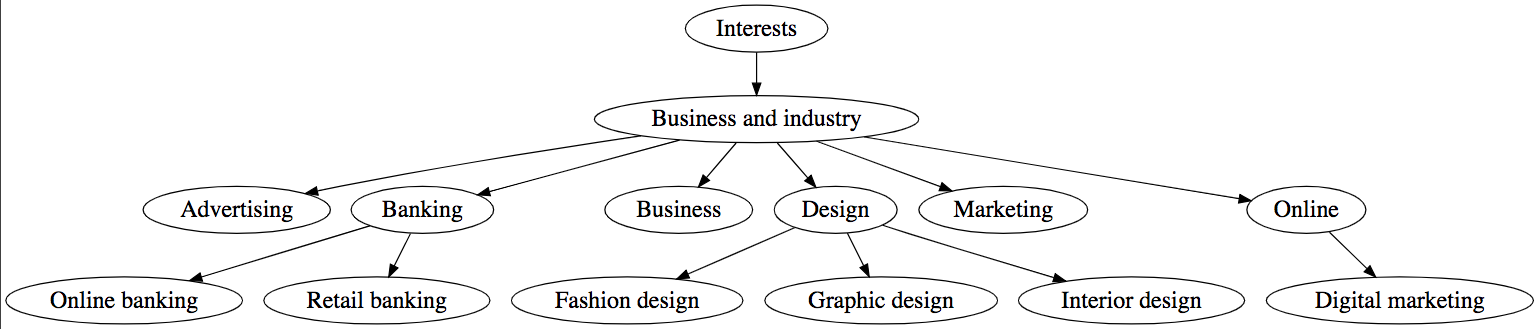
\includegraphics[width=150mm]{ontology.png}
    \caption{Caption}
    \label{fig:my_label}
\end{figure}

La ontología que ha creado Facebook se determina con un arbol de 8 intereses generales y 314 específicos cada uno clasificado según la relación a un interés general, esto nos permite buscar intereses específicos en común, por ejemplo si una persona le gustan los programas de televisión podemos asumir también que le gustan los reality shows o los programas de concursos etc, de esta forma otra persona que tenga un gusto de por ejemplo de series de televisión, tiene una relación directa con la primera y serán capaces de encontrar algún tema en común para iniciar una conversación.

% It may also be important to explain the ontology by indicating its parts and how interest of a branch may be related to one in another branch

\section{CEFR}

Conocida como \textbf{Common European Framework of Reference for Languages} por sus siglas en Inglés, es una herramienta usada a nivel internacional para evaluar el nivel de conocimiento de un idioma extranjero y es comúnmente conocido a lo largo del mundo de tal manera que aunque se haya realizado un test diferente, es posible encontrar un tipo de equivalencia usando esta clasificación, lo que nos permite ser capaces de tomar en cuenta en nivel de una persona sin importar que tipo de test tomo como información al registrarse en esta plataforma, o inclusive usando la descripción de cada uno de los niveles definirse a si mismo como perteneciente a alguno de ellos.
A continuación se describen los niveles y el significado de cada uno:

%\begin{itemize}
%\item \textbf{A1 - Principiante}: se dice que es capaz de usar expresiones comunes, dar información como su nombre, a que se dedican y donde viven. Y además pueden tener una interacción simple siempre y cuando la persona a la que se dirijan hable de forma clara y este preparada para ayudar.
%\item \textbf{A2 - Elemental: }
%\item \textbf{B1: Intermedio:}
%\item \textbf{B2: Intermedio Avanzado:}
%\item \textbf{C1: Avanzado:}
%\item \textbf{C2: Maestro:}
%\end{itemize}


